\chapter{Analyse}
Im folgenden Kapitel wird die Analyse der Netzwerksicherheit in Industrie 4.0 Umgebungen durchgeführt. Es wird eine Beschreibung und Einordnung der Bedrohungen von Industrie 4.0 Systemen anhand der in \autoref{Grundlagen:Grundprinzipien der sicheren Kommunikation} genannten Schutzziele und der aktuellen Industriestandards \autoref{Grundlagen:Normen und Standards} durchgeführt. Dabei wird nach den Schichten des \ac{TCP}/\ac{IP} Referenzmodells vorgegangen, um eine strukturierte Vorgehensweise zu ermöglichen und ein ganzheitliches Bild der Netzwerkkommunikation zu erhalten. Die Analyse wird mit Hilfe des Industrie 4.0 Testsystems (\cite{Weber2018}) durchgeführt. Dieses wird genutzt und erweitert, um verschiedene Szenarien darzustellen und die Sicherheit der Netzwerkkommunikation mit Hilfe verschiedener Softwaretools und Vorgehensweisen zu analysieren.

\section{Bedrohungen}
Die vierte industrielle Revolution, das \ac{IIoT} und dessen Vielzahl an aktiven und passiven Elementen stellen in ihrer Komplexität eine große Herausforderung für die IT-Sicherheit dar. Einerseits muss die Sicherheit der laufenden Software, der Infrastruktur, Anwendungs- und Rechnersysteme gewährleistet werden, andererseits muss die Betriebssicherheit der Geräte und Anlagen, welche mit dem Internet verbunden sind sichergestellt werden. Das Management der IT-Sicherheit in Industrie 4.0 Netzen geht über Unternehmensgrenzen hinweg, da Netze und Systeme für Kunden, Lieferanden und Partner bereitgestellt werden (\cite{DTAG2016}). Somit hat sich auch die Bedrohungslage der Netze geändert. Das \ac{BSI} beschreibt die Top 10 Bedrohungen und deren Folgen für \ac{ICS} in \cite{ICSSec2016}.

\begin{enumerate}
    \item Social Engineering und Phishing
    \item Einschleusen von Schadsoftware über Wechseldatenträger und externe Hardware
    \item Infektion mit Schadsoftware über Internet und Intranet
    \item Einbruch über Fernwartungszugänge
    \item Menschliches Fehlverhalten und Sabotage
    \item Internet-verbundene Steuerungskomponenten
    \item Technisches Fehlverhalten und höhere Gewalt
    \item Kompromittierung von Extranet und Cloud Komponenten
    \item \ac{DoS} und \ac{DDoS}
    \item Kompromittierung von Smartphones im Produktionsumfeld
\end{enumerate}

TODO - passt irgendwie nicht! - Bezug fehlt

Um die in \autoref{Grundlagen:Grundprinzipien der sicheren Kommunikation} genannten Schutzziele umzusetzen, ist es notwendig einen größtmöglichen Schutz gegen diese Bedrohungen bereitzustellen. Die Sicherheit eines Gesamtsystems kann nicht nur an einer einzigen Stelle im Kommunikationsstack hergestellt und gewährleistet werden. Es müssen alle Stellen des Kommunikationsstacks gegen Bedrohungen abgesichert werden (\cite{sichKom2017}). Dafür müssen die Netzwerkinfrastruktur und die eigentliche Kommunikation im Netzwerk gesichert werden. Dies geschieht durch die Abschottung von Systemen, die Einschränkung von Zugangsberechtigungen, die Härtung der Sicherheit der genutzten Komponenten sowie den Einsatz von geeigneten Netzwerkprotokollen und Verschlüsselungsverfahren.

\section{Netzzugangsschicht}
Die Netzzugangsschicht stellt die erste Instanz der Kommunikation in einem Netzwerk dar. Sie beinhaltet das Übertragungsmedium sowie die Topologie, in welcher die Kommunikation stattfindet. Das Übertragungsmedium bestimmt die Form der Signalübertragung. In Industrie 4.0 Netzen können neben der klassischen Kabelverbindung auch andere (instabile) Kanäle wie Mobilfunk oder Satelliten in Frage kommen. Um die Kommunikation über alle Medien sicher und zuverlässig zu gestalten, müssen auf technischer Ebene Protokolle genutzt werden, welche es ermöglichen die gegebenen Schutzziele zu realisieren und die Integrität der Daten bei der Übertragung über große Entfernungen zu gewährleisten. Dominante Technologien dieser Schicht sind \ac{IEEE} 802.3 (Ethernet)\footnote{Link zu IEEE 802.3}, \ac{IEEE} 802.11 (Wireless LAN)\footnote{Link zu IEEE 802.11} und \ac{IEEE} 802.15.4\footnote{Link zu IEEE 802.15.4} (\cite{sichKom2017}).

Aus zeitlichen Gründen wird keine weitere Analyse der verschiedenen Übertragungsmedien und deren Protokolle durchgeführt und sich im Rahmen dieser Thesis auf die Analyse von kabelgebundenen Ethernet-basierten Netzen, deren Topologie und Kommunikation beschränkt.

\subsection{physikalischer Zugang}
Die Netzzugangsschicht beinhaltet als einzige Schicht des \ac{TCP}/\ac{IP} Referenzmodells nicht nur die verwendeten Protokolle zur Signalübertragung, sondern auch die physikalischen Gegebenheiten des Übertragungsmediums. Die Sicherheit dieser Netzwerkschicht beinhaltet somit nicht nur die verwendeten Techniken, sondern auch die physische Sicherheit der Systeme. Sie wird durch den Zugang zur Hardware dargestellt und besitzt eine große Bedeutung, um unbefugte Eingriffe in das Netzwerk zu verhindern. Die Sicherheit dieser Systeme wird durch die physikalische Abschottung mit Hilfe von abschließbaren Serverschränken, genereller Zugangskontrolle sowie der Abschaltung von Ports an Netzwerkkomponenten oder Endsystemen gewährleistet. (\cite{sichKom2017})

\subsection{Topologie}
Die Topologie eines Netzwerks bestimmt den physikalischen Weg der Netzwerkpakete über die Leitungen. In der Industrie werden je nach Anwendungsfall verschiedene Topologien, wie Punkt-zu-Punkt-, Bus-, Stern- oder auch Hybride-, zur Kommunikation im Netzwerk genutzt. Jede dieser Netzstrukturen bietet Vor- und Nachteile bzgl. Durchsatz, Administrationsaufwand und Skalierbarkeit (\cite{burke2013}). Um die Grundidee der Industrie 4.0, die unternehmensübergreifende, intelligente Vernetzung von Produktionsressourcen umzusetzen, ist eine einheitliche Kommunikation notwendig. Industrie 4.0 Netze kommunizieren über \ac{TCP}/\ac{IP} Verbindungen und basieren auf dem \textit{Ethernet}\footnote{Link zu IEEE Ethernet} Protokoll. Sie werden in über Gateways miteinander verbundenen Sterntopologien realisiert. Die Topologie eines Netzwerks bietet Schnittstellen, um Einfluss auf das Netzwerk zu nehmen. Selbst unbefugter Zugriff auf der untersten Schicht des \ac{TCP}/\ac{IP} Referenzmodells kann die Sicherheit der Datenübertragung oder die Funktionsweise des Netzwerks beeinträchtigen.

TODO - Beschreibung von Angriffen durch Eingriff auf Hardware; Verweis auf Anwendungsszenario in Internetschicht.
TODO - Ansatz: Berechnung von Latenzzeiten, RTT, Auswirkungen aufzeigen, Congestion Window, Sliding Window

\subsection{\ac{VLAN}}
\label{Analyse:VLAN}
TODO - Taggen von Frames, da keine Kommunikation im Schichtenmodell zwischen den Schichten stattfindet. Somit QoS schwierig, da es von allen Hardwarekomponenten unterstützt werden muss und nicht nur auf Anwendungsebene funktionieren kann.

\subsection{ARP}
TODO - praktisch nur wenn Tool vorhanden ist.

\subsection{vertikale Integration bestehender Komponenten}
TODO - Feldbus, SPS, Anlagensteuerung (SCADA) -> Bindeglied zu IP-Netzen
TODO - Ansatz: OPC UA Clients sind Gateways in Testumgebung -> Verweis auf Analyse in höheren Schichten
TODO - Vieles in Praxis nicht umsetzbar darum größtmöglicher Schutz durch Abschottung.

\section{Internetschicht}
Auf der Internetschicht findet die Vermittlung der Datenpakete zwischen den Teilnehmern im Netzwerk statt. Auf dieser Schicht hat sich, mit dem Siegeszug des Internets, \ac{IP} zum Standard für Netzwerkübergreifende Rechnerkommunikation durchgesetzt (\cite{meinel2011}). Dies gilt auch für die immer komplexer werdenden Industrienetzwerke und die Industrie 4.0.

Zu den Aufgaben der Internetschicht gehört das Bereitstellen von Adressen, das Routing, die Fragmentierung von Datenpaketen zur Übertragung im Netzwerk sowie die Sicherstellung der Dienstgüte. Um Routing und Adressvergabe in \ac{IP}-Netzen zu realisieren, werden die Dienste \ac{DNS} und \ac{DHCP} genutzt. Das \ac{IPAM} und die Zuordnung der physikalischen Hardware zur logischen \ac{IP}-Adresse erfolgt mit Hilfe des \ac{ARP}. Da die Kommunikation in einem \ac{IP}-Netz ohne diese Dienste und Protokolle nicht möglich ist, stellen sie einen wichtigen Bestandteil der Kommunikation im Netzwerk da und müssen vor Sabotage geschützt werden.

\subsection{\ac{DNS}}
\ac{DNS} wird von der \ac{IETF} in den \ac{RFC} 1034\footnote{Domain Names – Concepts and Facilities}, 1035\footnote{Domain Names – Implementation and Specification}, 2181\footnote{Clarifications to the DNS Specification} und 2782\footnote{A DNS RR for specifying the location of services (DNS SRV)} beschrieben und verwaltet. Es stellt einen hierarchischen Verzeichnisdienst für \ac{IP}-Netze zur Verfügung. 

Eine der Hauptaufgaben des \ac{DNS} ist der \textit{forward lookup}. Hierbei werden Domain- bzw. Hostnamen in \ac{IP}-Adressen übersetzt. Das Zusammenspiel eines hierarchischen Verzeichnisdienstes und der Namensauflösung bietet Angriffsfläche zum Eingriff auf die Kommunikation im Netzwerk. Im folgenden werden bekannte Angriffsformen auf den \ac{DNS} Dienst und deren Auswirkungen auf das Netzwerk beschrieben.

\subsubsection{\ac{DNS} Spoofing}
Die Angriffsmethode des \ac{DNS} Spoofing verfolgt, wie \textit{Cache Poisoning}\footnote{Cache Poisoning - iwas}, das Ziel gefälschte \ac{RR} in den \ac{DNS} Cache des Opfers einzuschleusen. Während das \textit{Cache Poisoning} aus einer Softwareschwachstelle hervorging, bei der zusätzliche, gefälschte \ac{DNS} Einträge zu korrekten \ac{DNS} Antworten hinzugefügt wurden und somit der Cache eines Nameservers kompromittiert wird, befindet sich der Angriffsvektor beim \ac{DNS} Spoofing in der Fälschung von \ac{DNS} Antworten. Der Header der Netzwerkpakete werden mit Hilfe von \textit{IP Spoofing}\footnote{IP Spoofing bezeichnet das Versenden von IP Paketen mit gefälschter Absender-IP} so manipuliert, dass sie vorgeblich vom \textit{authorativen} Nameserver stammen. 

Um \ac{DNS} Spoofing erfolgreich durchzuführen muss die gefälschte \ac{DNS} Response des Angreifers vor der Antwort des zuständigen Nameservers beim angegriffenen \ac{DNS} Resolver eintreffen. Sobald der physikalische Zugang zum Netzwerk gewährleistet ist, können die Latenzzeiten der gefälschten Pakete im Netzwerk sehr gering gehalten werden. Ist dies nicht möglich, kann mit Hilfe eines \ac{DoS} bzw. \ac{DDoS} Angriffs (siehe \autoref{Analyse:DoS/DDos}) auf den zuständigen Nameserver, dessen Antwortzeit beeinflusst werden. Des weiteren muss die ID im \ac{DNS} Header mit der des Request übereinstimmen. Dies kann am Testsystem am Beispiel der Namensauflösung des \ac{OPC UA} Discovery Servers mit Hilfe des Netzwerkanalysetools Wireshark\footnote{Link zu Wireshark} nachgewiesen werden.

\begin{figure}[h]
    \centering
    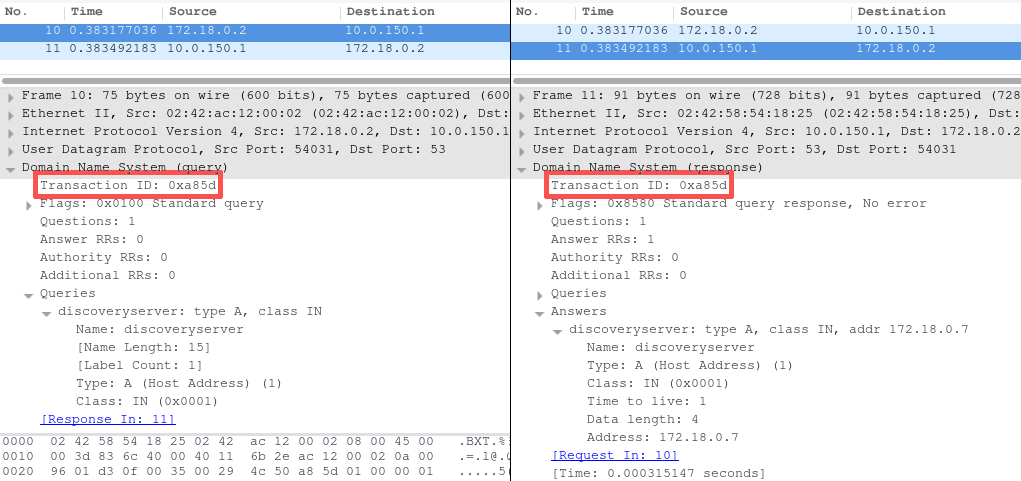
\includegraphics[width=15cm]{dns-response-request}
    \caption{Wireshark - ID im DNS Header}
    \label{Analyse:DNS Request Response}
  \end{figure}
  
\clearpage

In der Darstellung ist auf der linken Seite ein DNS Request des \ac{OPC UA} Discovery Servers und dessen DNS Header mit ID zu erkennen. Auf der rechten Seite ist die Antwort des im Netzwerk vorhandenen authorativen Nameservers zu sehen.

\subsubsection{\ac{DNS} Amplification}
Eine Form eines \ac{DDoS} Angriffs (\autoref{Analyse:DoS/DDos}) ist über \ac{DNS} möglich und wird \ac{DNS} Amplification genannt. Bei der \ac{DNS} Amplification werden \ac{DNS} Anfragen an offene Nameserver gesendet und mit Hilfe von \ac{IP} Spoofing als Quell-\ac{IP} die Adresse des Angreifers genutzt. Somit treffen die \ac{DNS} Antworten beim anzugreifenden System ein und belasten dieses durch erhöhten Rechenaufwand sowie dessen Netzwerk durch Traffic. Ein weiterer Seiteneffekt dieses Angriffs ist eine hohe Last der Nameserver, welches durch das rekursive Verhalten der \ac{DNS} Namensauflösung hervorgerufen wird. \ac{DNS} Amplification bezeichnet eine Form des \ac{DRDoS}.

Mit der Erweiterung des \ac{DNS} in der \ac{IETF} \ac{RFC} 2617\footnote{Link - https://www.ietf.org/rfc/rfc2671.txt} wurde es notwendig, die Größe der \ac{DNS} Antworten von 512 Byte auf einen dynamischen Puffer bis über 4000 Bytes zu erhöhen, um zusätzliche Informationen und Flags wie \autoref{Analyse:DNSSEC} über das \ac{DNS} übertragen zu können. Dies wird sich vom Angreifer zunutze gemacht, da an den Nameserver Requests mit einer Paketgröße von 60 Bytes gesendet werden können, welche eine Antwort mit 4000 Bytes und mehr provozieren und somit einen \ac{BAF} von ca. 66 im Netz haben. \cite{Ledermueller2009}. Der \ac{BAF} beschreibt das Verhältnis von Eingang- zum Ausgangssignal. Dies wird bei \ac{DNS} Amplifikation durch die Paketgröße der Anfrage sowie der Antwort dargestellt.

Die folgende Abbildung stellt einen \ac{DDoS} Angriff durchgeführt durch \ac{DNS} Amplification schematisch dar. Der Angreifer (links) sendet zu zwei offenen Nameservern gefälschte \ac{DNS} Anfragen mit Quelladresse des Opfers (rechts). Die offenen Nameserver erfragen beim authorativen Nameserver die Zone, dieser stellt die erfragten \ac{RR} bereit und die offenen Nameserver senden dem Opfer Antworten zu.

\begin{figure}[h]
    \centering
    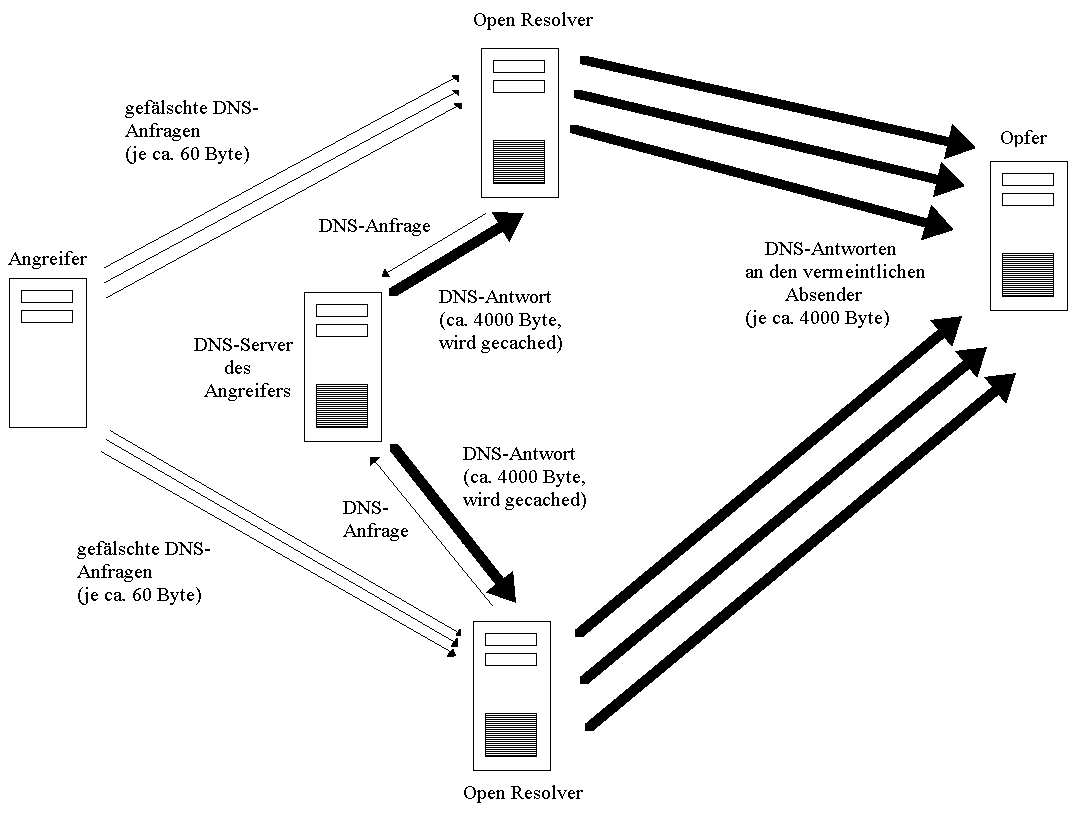
\includegraphics[width=15cm]{dns-amplification}
    \caption{Schematisches Beispiel: DNS Amplification}
    \label{Analyse:DNS Amplification}
  \end{figure}
  
\clearpage

Diese Form des Angriffs kann aus dem internen Netz sowie von extern auf öffentlich zugängliche Systeme durchgeführt werden. \ac{DoS} Attacken stellen besonders für Industrie 4.0 Netzwerke, deren komplexe Kommunikation und Anforderungen eine hohe Bedrohung dar. Durch den erheblichen \ac{BAF} können diese Angriffe mit wenig Bandbreite beim Angreifer durchgeführt werden und gleichzeitig das Netzwerk des Opfers voll auslasten. Dies wird im folgenden anhand einer Grafik dargestellt. 

TODO - Beschreibung -> Plot Netzlast Angreifer - Netzlast Opfer - Skalierung

Der \ac{DNS} bietet weitere Angriffsmöglichkeiten wie \ac{DNS} Fast Fluxing oder \ac{DNS} Information Leakage. Diese Angriffe dienen zum \textit{Phishing} von Daten oder der Spionage der Netzwerkstruktur. Sie nehmen initial keinen Einfluss auf den Netzwerkverkehr und dienen der Vorbereitung von Folgeangriffen und dem Sammeln von Informationen. Die Angriffsformen werden in \cite{Ledermueller2009} näher beschrieben. Die Analyse der Sicherheit der Netzwerkkommunikation beschränkt sich auf Angriffe, welche direkten Einfluss in die Kommunikation im Netzwerk haben. Weitere Formen der \ac{DoS}/\ac{DDoS} Angriffe finden auf Transportschicht \autoref{Analyse:Transportschicht} durch \textit{SYN-Flooding} oder auf Anwendungsschicht \autoref{Analyse:Anwendungsschicht} zur Negierung eines Speziellen Dienstes statt.

TODO - Schutzmaßnahmen sind DNSSEC und zufällige Informationen \label{Analyse:DNSSEC}
TODO - Die Auswirkungen eines solchen Angriffs ...
TODO - Sicherheitsmaßnahmen siehe \cite{Ledermueller2009}

\subsection{\ac{QoS}}
Eine Industrie 4.0 Netzwerkinfrastruktur kann aufgrund der unterschiedlichen Anforderungen an die Systeme auf verschiedenste Weisen ausgeprägt sein. Die Heterogenität der Komponenten im Netzwerk und deren Anforderungen an die Kommunikation auf der vertikalen Ebene der Automatisierungspyramide \autoref{Grundlagen:Automatisierungspyramide} stellen eine Herausforderung für die Sicherheit der Datenübertragung dar und können die Umsetzung eines Netzwerks beeinflussen. Des Weiteren erstrecken sich Industrie 4.0 Umgebungen über weite Distanzen (\ac{MAN}, \ac{WAN}, \ac{GAN}) und sind somit auch von physikalischen Gegebenheiten wie Latenz und Jitter betroffen. Diese Erscheinungen müssen berücksichtigt werden, um eine fehler- und verlustfreie, sichere Kommunikation zu gewährleisten \cite{torscht2014}.

Für die Beurteilung und Bereitstellung der Dienstgüte in \ac{IP}-Netzen müssen die Übertragungsgüte der Netzzugangsschicht sowie die übertragungstechnischen Parameter der Internetschicht (\ac{IP}-Ebene) betrachtet werden. In IP-Netzen wird der Einfluss auf die \ac{QoS} in den folgenden Parametern beschrieben:
\begin{itemize}
    \item Latenzzeit: Dauer der Paketübertragung
    \item Jitter: Abweichung der Latenzzeit von ihrem Mittelwert
    \item Paketverlustrate: Wahrscheinlichkeit des Verlusts von IP-Paketen während der Übertragung
    \item Durchsatz: gemittelte Datenmenge pro Zeiteinheit
\end{itemize}
All diese Faktoren haben in einem paketorientierten Netzwerk, in welchem die Datenpakete nach dem \textit{Best-Effort-Prinzip} versendet werden, auf die fehlerfreie Kommunikation aufgrund der durch \textit{Ethernet} und \ac{IP} bereitgestellten Fehler- und Flusskontrolle wenig Einfluss. Sie spielen jedoch bei zeitkritischen Anwendungen der Industrie 4.0 eine wichtige Rolle. Auf den niedrigeren Schichten des \ac{TCP}/\ac{IP} Referenzmodells ist es nicht möglich zwischen verschiedenen Datenpaketen der höheren Schichten zu unterscheiden. Um dieses Problem zu lösen werden auf Dienste mit besonderer Güte in \ac{VLAN}s aufgenommen und somit deren Pakete bereits auf der Netzzugangsschicht kenntlich gemacht (\autoref{Analyse:VLAN}), um die Dienstqualität sicherzustellen. Des Weiteren müssen, um \ac{QoS} in einem Netzwerk anzuwenden, diese Mechanismen auf der gesamten Übertragungsstrecke implementiert werden. Der Transport von Daten unterschiedlicher Priorität in Netzwerken wird in \ac{IEEE} 802.1p und \ac{IEEE} 802.1Q\footnote{IEEE Std 802.1Q - IEEE Standard for Local and metropolitan area networks--Bridges and Bridged Networks} beschrieben.

\subsection{IPsec}
TODO - Die Internetschicht bietet mit IPsec eine Möglichkeit den Datenfluss, im Vergleich zu anderen Verschlüsselungsverfahren, bereits auf der Internetschicht des \ac{TCP}/\ac{IP} Referenzmodells zu sichern.

\section{Transportschicht}
\label{Analyse:Transportschicht}
TODO - Einleitung -> Protokolle der Transportschicht hängen von Kommunikationsstruktur und Anforderungen ab.

\subsection{Kommunikationsstrukturen in Industrie 4.0 Umgebungen}
Um die Kommunikation zwischen verschiedenen Teilnehmern zu ermöglichen, ergeben sich in der Praxis unterschiedliche Strukturen. Jede dieser Strukturen bietet, je nach Anwendungsfall und zu erfüllenden Anforderungen, Vor- und Nachteile.

\subsubsection{End2End}
Die Komponenten der Industrie 4.0 Umgebung kommunizieren über einen direkten Kanal miteinander. Dies setzt voraus, dass sich beide Teilnehmer in einem Netzwerk befinden, welches die benötigten Dienste wie z. B. \ac{IP} und \ac{DNS} zur Kommunikation bereitstellt. Des weiteren müssen beide Systeme diese Dienste und Protokolle unterstützen.

\subsubsection{Gateways}
Um existierende Systeme, welche selbst nicht Industrie 4.0 konform kommunizieren oder zu wenig Rechenleistung besitzen, in die Industrie 4.0 Welt zu integrieren, werden Industrie 4.0 Gateways genutzt. Dabei ist jedoch zu beachten, dass die Systeme hinter den Gateways nicht als Industrie 4.0 Komponenten entwickelt wurden und somit auch keine oder nur wenige dieser Eigenschaften besitzen. Des Weiteren ist es möglich, dass die Kommunikation aus Leistungsgründen oder besonderer Anforderungen über optimierte, proprietäre Protokolle stattfindet. Die Gateways müssen auf die Systeme und deren Protokolle individuell konfiguriert werden, um die Funktionalitäten im Industrie 4.0 Netz bereitstellen zu können, und die Kommunikation zu schützen.

\subsubsection{Publish-Subscribe}
Das Publish-Subscribe Modell bietet die Möglichkeit Informationen an mehrere Teilnehmer zu verteilen. Hierbei melden sich die Empfänger beim Verteiler an und wählen aus, über welche Nachrichtentypen sie informiert werden möchten. Diese Verteildienste nutzen zur besseren Skalierung und Reduzierung der Netzlast häufig Datagramme wie \ac{UDP}. Durch die Nutzung von Datagrammen geht jedoch die Fehlertoleranz verloren. Somit muss entweder dafür gesorgt werden, dass eine sehr zuverlässige Netzwerkinfrastruktur vorhanden ist und hohe Bandbreitenreserven geschaffen werden, um die Dienstgüte (\ac{QoS}) sicherzustellen oder dieses Modell nur für fehlertolerante Kommunikation wie z. B. Audio- und Video-Anwendungen oder Businessprozesse zu nutzen. 

\subsubsection{Kommunikation mit Netzwerk als Partner}
Zeitkritische Automatisierungsanwendungen verlangen besondere Netzwerkeigenschaften. Sie können auf Latenz oder Jitter angewiesen sein. Um diese Eigenschaften sicherzustellen, ist es sinnvoll in diese Netze eine Industrie 4.0 Schnittstelle zu integrieren. Somit ist es den Teilnehmern möglich, über die Verwaltungsschale sicherzustellen, dass das Netzwerk die erforderlichen Anforderungen bereitstellt. \cite{sichKom2017}

TODO - Bilder -> sichere-kommunikation-i40
TODO - mehr Analyse.

\subsection{TCP}
\subsection{UDP}

TODO - Verweis auf \autoref{Analyse:Anwendungsschicht}, da Tests mit OPC UA auch Transportschicht umfassen. -> PubSub, Client-Server = UDP/TCP

\section{Anwendungsschicht}
\label{Analyse:Anwendungsschicht}
TODO - Einleitung

\subsection{Integrationsansätze}
Die Grundlage der Industrie 4.0 Kommunikation ist ein standardisierter Datenaustausch über alle Schichten der Automatisierungspyramide hinweg. Dabei stellt der \ac{IEC}-Standard \ac{OPC UA} einen vielversprechenden Ansatz für einen standardisierten Informationsaustausch über Unternehmensgrenzen hinweg dar. Jedoch müssen auch bestehende Systeme in die Industrie 4.0 Kommunikation integriert werden. Dies führt häufig zu Problemen, da diese Systeme proprietäre Protokolle nutzen, besondere Anforderungen wie Echtzeitkommunikation besitzen oder gar keine Schnittstelle bereitstellen. Es bestehen grundsätzlich zwei Ansätze zur Integration dieser Anlagen. TODO - ref.

\subsubsection{Konsolidierung der Netzwerkkommunikation}
TODO - Eine Möglichkeit der Entwicklung zu einer Smart Factory ist die Konsolidierung die Netzwerkkommunikation. Fokus auf OPC UA, da standardisiert.
TODO - neue Netze/Factories können so geplant werden, dass die Maschinen die benötigten Schnittstellen bereitstellen.
Ansatz: teuer, aufwendig bzw. nicht möglich, da embedded System bzw. keine Ressourcen oder keine Schnittstellen

\subsubsection{Gatewaykommunikation}
Eine Alternative zur Umstellung der bestehenden Systeme stellt die Kommunikation über Gateways dar. Hierbei gibt es mehrere Softwarelösungen, welche unterschiedliche Ziele verfolgen. Es werden Systeme zur Anlagenoptimierung (TODO - ref. SePiA.Pro), der Bereitstellung einer offenen, branchenübergreifenden Plattform mit diversen Smart Services wie Datenanalyse und Flottenmanagement (TODO - ref. Siemens Mindsphere, DeviceInsight) und dem herstellerübergreifenden Gerätemanagement (AXOOM) entwickelt \cite{acatec2016}. Die Systeme sammeln und verwalten die Daten der Anlagen an zentraler Stelle und stellen sie im Netzwerk zur Verfügung. Der Einsatzmöglichkeiten dieser Softwarelösungen sind von den vorhandenen Schnittstellen der Anlagen abhängig und benötigen eine individuelle Konfiguration um den unterschiedlichen Anforderungen der Industrielandschaft gerecht zu werden.

TODO - Im folgenden Abschnitt wird die Umsetzung der Kommunikation über eine digitale Serviceplattform am Beispiel von AXOOM dargestellt. eher nicht!

\paragraph{AXOOM}
TODO - 2016 Innovationspreis deutsche Indsutrie
TODO - unterstützt Optimierung der Wertschöpfungskette -> ERP-, MES Kommunikation über "bekannte", offene Schnittstellen (REST usw.) 
TODO - unterstützt Anbindung von \ac{IoT}. Analyse und Visualisierung von Daten -> Kommunikation über spezielle Schnittstellen
TODO - sichere Kommunikation durch AXOOM Gate - wie? Quellen? -> "Dieses basiert teilweise auf Technologien unseres Partners C-Labs und schafft eine direkte Verbindung zwischen dem Kundennetzwerk und der Cloud. Das AXOOM Gate ist in der Lage, Daten herstellerunabhängig von allen angebundenen Geräten zu sammeln, so dass diese verschlüsselt an die AXOOM Plattform gesendet und dort visualisiert und ausgewertet werden können. Besonderen Schutz bei der Datenübertragung bietet ein mehrstufiges Sicherheits- und Verschlüsselungskonzept auf Komponenten-, Transport-, Applikations- und Anwenderebene. So wird eine genaue Zugriffskontrolle innerhalb der Fabrik sowie auf die Fabrik sichergestellt, unsichere Verbindungen von und nach Außen sind ausgeschlossen."
TODO - offene Schnittstellen für Low Level
TODO - REST usw. für High Level Applications
TODO - Softwareschwachstellen, Softwarefehler 
TODO - Herstellerabhängigkeit
TODO - Kosten der Interfaceentwicklung, usw.

\subsection{DHCP}
TODO - Beschreibung

In Kapitel \autoref{Impl:DHCP Spoofing} wird die Erweiterung des Testsystems (\cite{Weber2018}) beschrieben und Auswirkungen eines Eingriffs auf das Netzwerk in der Netzzugangsschicht und gleichzeitige Manipulation des \ac{DHCP} der Anwendungsschicht des \ac{TCP}/\ac{IP} Referenzmodells dargestellt.

\subsection{\ac{DDS}}
TODO - Beschreibung

\subsection{\ac{OPC UA}}
TODO - siehe BSI UPC UA Analyse.
TODO - The OPC UA specifications are layered to isolate the core design from the underlying computing technology and network transport. This allows OPC UA to be mapped to future technologies as necessary, without negating the basic design. Mappings and data encodings are described in Part 6. Three data encodings are defined:
\begin{itemize}
    \item XML/Text
    \item UA Binary
    \item JSON
\end{itemize}
In addition, several protocols are defined:
\begin{itemize}
    \item OPC UA TCP
    \item HTTPS
    \item WebSockets
\end{itemize}

TODO - ref. OPC Pt. 1
TODO - \ac{OPC UA} ist in der \ac{IEC} 62541 als offener Standard definiert und erstreckt sich über Communication- und Information Layer des \ac{RAMI4.0}, da es eine \ac{SOA} bereitstellt. 
TODO - vereint Daten und Informationsdienste. 

\begin{figure}[h]
    \centering
    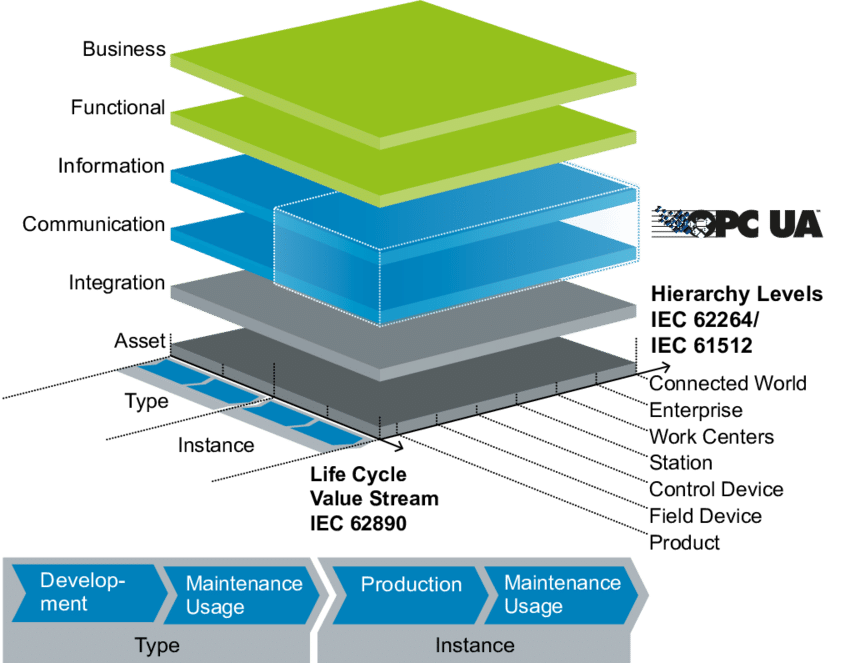
\includegraphics[width=15cm]{opcua_rami40}
    \caption{OPC UA im RAMI 4.0}
    \label{Kap3:OPC UA im RAMI 4.0}
  \end{figure}
\clearpage

\subsection{MQTT/CoAP}
TODO - Ansatz: Wireshark an Bridge der Testumgebung im Sternnetzwerk und Druckerkomponente oder andere manipulieren; andere Protokolle von Feldebene an Switch auslesen; vielleicht hier nur beschreiben und in den höheren Schichten durchführen mit CoAP oder MQTT -> OPC UA Komponenten sind Gateway

\section{Schutzmaßnahmen}
TODO - Applikationssicherheit != Netzwerksicherheit != Betriebssystemsicherheit
TODO - Schutz auf allen Ebenen -> z.B. OPC UA basiert auf IP-Netz -> Angriffsvektoren von IP und genutzten Diensten immer noch zutreffend
\subsection{Allgemeine Maßnahmen}
\subsection{TODO}
\subsection{Defense in Depth}
Auf der Netzzugangsschicht fallen, wie auf allen anderen Schichten, Betriebsdaten an, welche genutzt werden können, um Angriffe oder unregelmäßige Aktivitäten im Netzwerk zu erkennen. Es kann protokolliert werden, wann ein Gerät mit den Netzwerk verbunden war und welche Pakete andere Netzwerkteilnehmer von diesem Gerät erhalten haben (\cite{sichKom2017}). Die Norm IEC 62443\footnote{ref. IEC 62443} definiert die Defense in Depth Strategie. Sie stellt ein Konzept bereit, um die IT-Sicherheit der Anlagen, die Netzwerksicherheit und Systemintegrität nach dem Stand der Technik zu schützen. Sie gliedert eine Unternehmensinfrastruktur in multiple und redundante Sicherheitsschichten (Zonen), um ein höchstmögliches Sicherheitsniveau zu erreichen. Die unabhängigen Verteidigungslinien sollen Angriffe verzögern, um Zeit für Gegenmaßnahmen zu gewinnen. Die Kommunikation erfolgt in separierten Netzsegmenten, welche zusätzlich mit \ac{IDS} nutzen, um Angriffe schnell zu erfassen und Gegenmaßnahmen einleiten zu können. Somit wird der Aufwand, um die unteren Netzwerkebenen zu kompromittieren durch den Einsatz von \ac{DMZ}, \ac{IDS}, Paketfilter und Time Access Control wesentlich erhöht. Zusätzlich ist das "`Zone and Conduit"' Modell eines der zentralen Elemente der Defense in Depth Strategie. Die verschiedenen Zonen können nur mittels spezieller Leitungen (Conduits) miteinander kommunizieren.  

\begin{figure}[h]
    \centering
    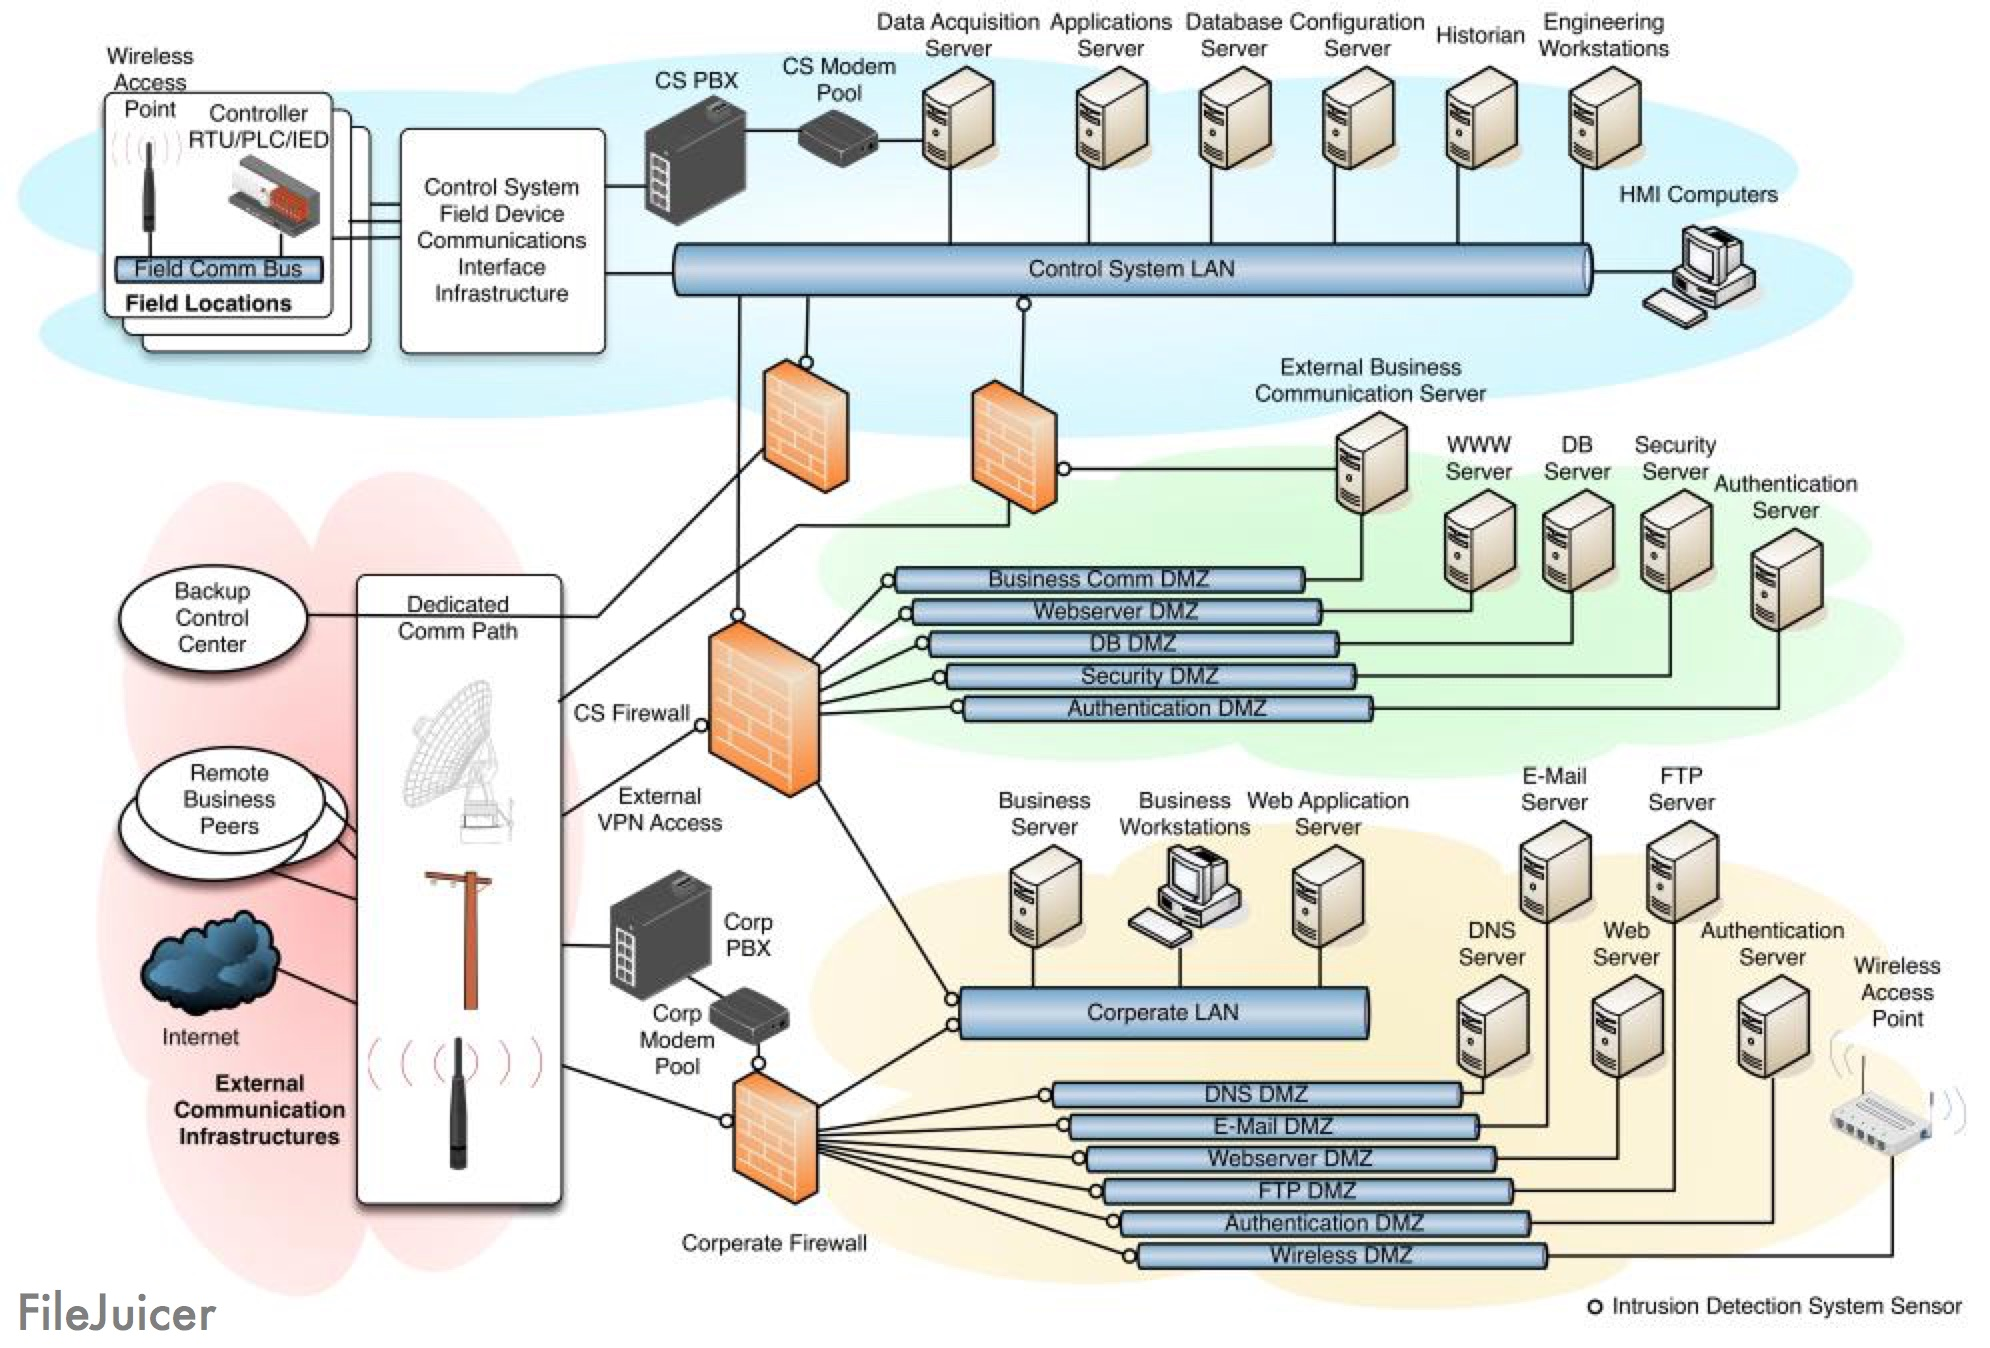
\includegraphics[width=15cm]{defense-in-depth-strategie}
    \caption{Defense in Depth Strategie - \cite{kuipers2006}}
    \label{Kap3:Defense-in-Depth}
\end{figure}

\clearpage

Das Defense in Depth Konzept stellt ein Konzept dar, um Industrieanlagen und Unternehmensnetzwerke vor Angriffen zu schützen. Bei der sich ständig ändernden Bedrohungslage in den komplexen Netzen wird bei dieser Strategie jedoch weniger ein vollständiger Schutz bereitgestellt, als eine Strategie zur Schadensbegrenzung im Falle eines Angriffs.

\section{Auswertung der Ergebnisse}
TODO